%!TEX program = xelatex
\documentclass[11pt,article,oneside]{memoir}
\usepackage{org-preamble-xelatex}
\DisemulatePackage{setspace}
\usepackage{setspace}
\usepackage{titling}
\setlength{\droptitle}{-12em}
% \input{vc}

\usepackage{longtable}

\usepackage{graphicx}
% We will generate all images so they have a width \maxwidth. This means
% that they will get their normal width if they fit onto the page, but
% are scaled down if they would overflow the margins.
\makeatletter
\def\maxwidth{\ifdim\Gin@nat@width>\linewidth\linewidth
\else\Gin@nat@width\fi}
\makeatother
\let\Oldincludegraphics\includegraphics
\renewcommand{\includegraphics}[1]{\Oldincludegraphics[width=\maxwidth]{#1}}

\title{How Does the State Speak about Globalisation? A Quantitative Text-Mining
Approach}

%\author{}

\author{\Large Justin Murphy\vspace{0.05in} \newline\normalsize\emph{University of Southampton} \newline\footnotesize \url{j.murphy@soton.ac.uk}\vspace*{0.2in}\newline }

%\author{Justin Murphy (University of Southampton)}

\date{}


\begin{document}  
\setkeys{Gin}{width=1\textwidth} 	
\setromanfont[Mapping=tex-text,Numbers=OldStyle]{Georgia} 
\setsansfont[Mapping=tex-text]{Gill Sans} 
\setmonofont[Mapping=tex-text,Scale=0.8]{Consolas}
\chapterstyle{article-jmrphy}
\pagestyle{kjh}

\singlespacing


\maketitle



\vspace{-4ex}
\begin{abstract}

\noindent Scholars argue that the concept of ``globalisation'' is strategically
deployed by governments to rationalise their policy choices (Hay and
Rosamond 2011). This article is the first large-scale quantitative
assessment of this argument, using text-mining and machine learning
techniques to analyze more than 60,000 government web pages.
Specifically, this article exploits the newly released United Kingdom
Government Web Archive to analyze a random sample of web pages published
across the entire UK government web system between 2000 and 2013.

\end{abstract}

\newpage


\subsection{Data}\label{data}

The UK Government Web Archive stores more than 7 terabytes of digital
items hosted across the UK government web system since 2000. These items
include a wide variety of web pages but also documents, such as Adobe
PDF files, hosted within the UK government web system.

The UK National Archives provides an API for programmatic web access to
the entire Web Archive. The API allows users to search the archive with
a basic set of search operators, and provides the full text as well as
some metadata for all items in the entire archive which match a given
search criteria. The returned results are not ordered according to any
principle so their ordering can be thought of as random.

Data collection began with an attempt to scrape 150,000 items from the
UK Government Web Archive API. Of the 150,000 attempted, 67,000 items
were successfully returned before the request timed-out. Of the returned
items, about 1,000 were empty due to connection errors. Thus, the sample
consists of a corpus containing 66,000 text documents.

\subsubsection{Descriptive Statistics}\label{descriptive-statistics}

\begin{figure}[htbp]
\centering
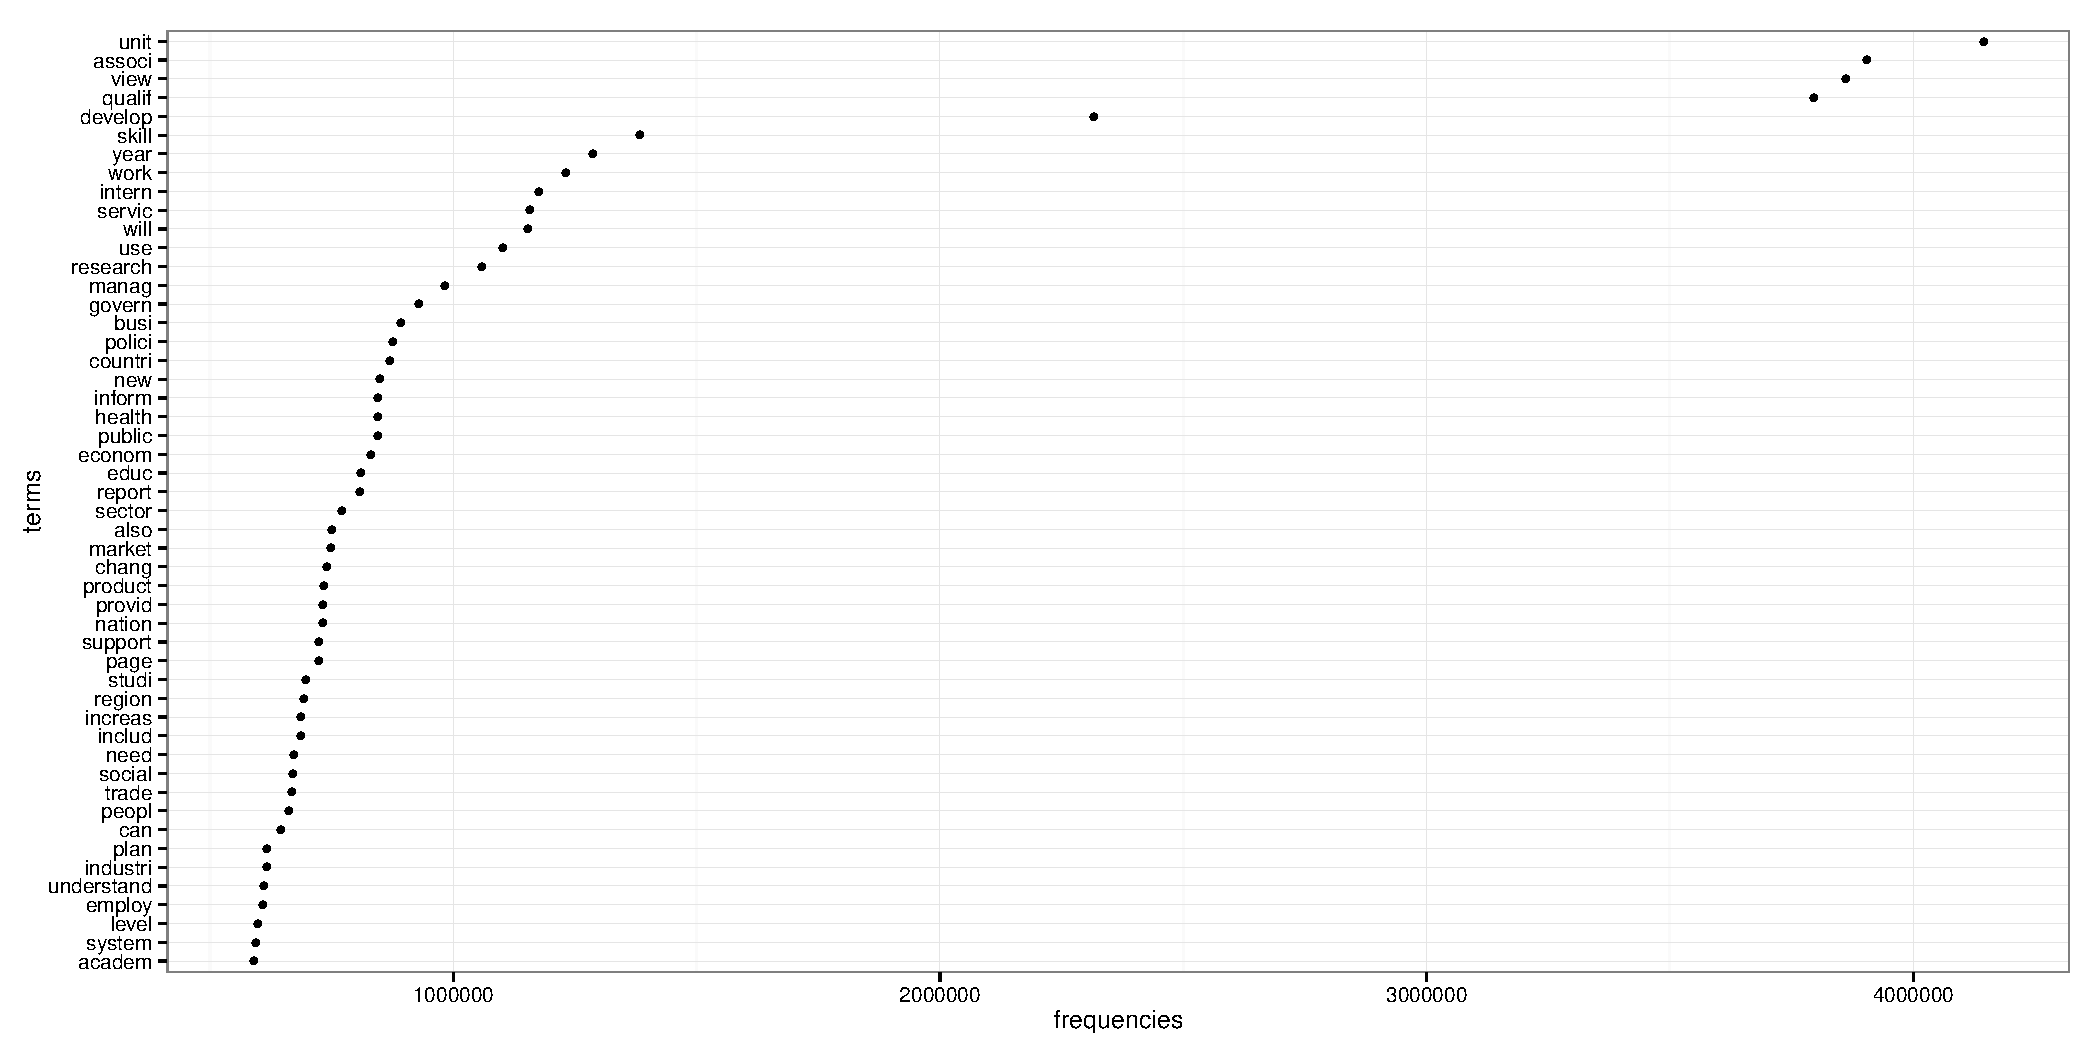
\includegraphics{figure/globalisation_frequency_plot.pdf}
\caption{Most Frequent Terms in Web Pages Containing ``Globalisation''}
\end{figure}

\pagebreak

\paragraph{Economic Terms}\label{economic-terms}

\begin{longtable}[c]{@{}lrlrlrlrlr@{}}
\toprule\addlinespace
global & r & capit & r.1 & wage & r.2 & inflat & r.3 & unemploy & r.4
\\\addlinespace
\midrule\endhead
world & 0.78 & account & 0.56 & abstract & 0.62 & monetari & 0.64 &
labour & 0.72
\\\addlinespace
countri & 0.66 & economi & 0.56 & paper & 0.62 & price & 0.51 & rate &
0.64
\\\addlinespace
economi & 0.63 & financi & 0.56 & download & 0.60 & fiscal & 0.46 & job
& 0.61
\\\addlinespace
threat & 0.62 & incom & 0.55 & seri & 0.60 & gdp & 0.45 & census & 0.55
\\\addlinespace
increas & 0.61 & expenditur & 0.54 & richard & 0.57 & macroeconom & 0.44
& month & 0.55
\\\addlinespace
goal & 0.60 & stabil & 0.54 & worker & 0.52 & rate & 0.43 & earn & 0.54
\\\addlinespace
key & 0.60 & debt & 0.51 & earn & 0.50 & output & 0.34 & percentag &
0.54
\\\addlinespace
agricultur & 0.59 & extern & 0.51 & revis & 0.50 & debt & 0.33 & spring
& 0.54
\\\addlinespace
also & 0.59 & market & 0.51 & labour & 0.42 & economi & 0.31 & win &
0.53
\\\addlinespace
develop & 0.58 & reduc & 0.51 & unemploy & 0.42 & quarter & 0.31 &
employ & 0.52
\\\addlinespace
particular & 0.57 & macroeconom & 0.50 & econom & 0.41 & growth & 0.29 &
januari & 0.51
\\\addlinespace
econom & 0.55 & also & 0.49 & rate & 0.37 & interest & 0.29 & vacanc &
0.51
\\\addlinespace
mani & 0.55 & flow & 0.49 & oecd & 0.35 & bulletin & 0.27 & adjust &
0.50
\\\addlinespace
privat & 0.55 & fund & 0.49 & union & 0.35 & gross & 0.27 & averag &
0.47
\\\addlinespace
coher & 0.54 & net & 0.49 & outlook & 0.34 & ratio & 0.27 & exclud &
0.47
\\\addlinespace
competit & 0.54 & spend & 0.49 & ratio & 0.32 & adjust & 0.26 & per &
0.45
\\\addlinespace
primari & 0.53 & strengthen & 0.49 & employ & 0.31 & billion & 0.26 &
cent & 0.44
\\\addlinespace
educ & 0.52 & econom & 0.48 & employe & 0.31 & estim & 0.26 & nov & 0.44
\\\addlinespace
exampl & 0.52 & commit & 0.47 & subscrib & 0.31 & oecd & 0.26 & age &
0.43
\\\addlinespace
howev & 0.52 & competit & 0.47 & estim & 0.29 & outlook & 0.26 & wage &
0.42
\\\addlinespace
integr & 0.52 & includ & 0.47 & job & 0.29 & percentag & 0.26 & week &
0.42
\\\addlinespace
success & 0.52 & interest & 0.47 & declin & 0.28 & stabil & 0.26 &
outlook & 0.40
\\\addlinespace
argu & 0.50 & invest & 0.46 & empir & 0.28 & incom & 0.25 & proport &
0.38
\\\addlinespace
capac & 0.50 & particular & 0.46 & effect & 0.27 & index & 0.25 & survey
& 0.38
\\\addlinespace
dfid & 0.50 & privat & 0.46 & growth & 0.27 & tax & 0.25 & men & 0.37
\\\addlinespace
millennium & 0.50 & benefit & 0.45 & incom & 0.27 & capit & 0.24 & sampl
& 0.37
\\\addlinespace
similar & 0.50 & full & 0.45 & market & 0.27 & bank & 0.23 & worker &
0.37
\\\addlinespace
impact & 0.49 & can & 0.44 & resid & 0.27 & revis & 0.23 & dec & 0.36
\\\addlinespace
can & 0.48 & ensur & 0.44 & survey & 0.27 & borrow & 0.22 & market &
0.36
\\\addlinespace
poverti & 0.48 & investor & 0.44 & economi & 0.26 & earn & 0.22 & econom
& 0.35
\\\addlinespace
\bottomrule
\end{longtable}

\pagebreak

\paragraph{Imperative Terms}\label{imperative-terms}

\begin{longtable}[c]{@{}lrlrlrlr@{}}
\toprule\addlinespace
requir & r & necessarili & r.1 & system & r.2 & threat & r.3
\\\addlinespace
\midrule\endhead
includ & 0.76 & howev & 0.68 & technolog & 0.64 & global & 0.62
\\\addlinespace
also & 0.75 & can & 0.67 & also & 0.63 & also & 0.61
\\\addlinespace
particular & 0.75 & like & 0.67 & can & 0.63 & countri & 0.57
\\\addlinespace
can & 0.72 & particular & 0.67 & integr & 0.63 & mani & 0.56
\\\addlinespace
howev & 0.71 & exampl & 0.66 & exampl & 0.61 & particular & 0.56
\\\addlinespace
exampl & 0.70 & mani & 0.66 & howev & 0.60 & world & 0.56
\\\addlinespace
similar & 0.70 & also & 0.65 & includ & 0.60 & goal & 0.54
\\\addlinespace
will & 0.69 & similar & 0.61 & particular & 0.59 & howev & 0.54
\\\addlinespace
within & 0.69 & just & 0.58 & requir & 0.59 & exampl & 0.53
\\\addlinespace
avail & 0.67 & import & 0.57 & reduc & 0.58 & coher & 0.51
\\\addlinespace
effect & 0.66 & argu & 0.55 & mani & 0.57 & privat & 0.51
\\\addlinespace
provid & 0.66 & evid & 0.55 & applic & 0.56 & success & 0.51
\\\addlinespace
ensur & 0.65 & may & 0.55 & similar & 0.56 & argu & 0.50
\\\addlinespace
level & 0.65 & requir & 0.54 & technic & 0.56 & educ & 0.50
\\\addlinespace
key & 0.62 & interest & 0.53 & order & 0.55 & primari & 0.50
\\\addlinespace
like & 0.62 & within & 0.53 & provid & 0.55 & similar & 0.50
\\\addlinespace
mani & 0.61 & avail & 0.52 & avail & 0.54 & capac & 0.49
\\\addlinespace
refer & 0.61 & question & 0.52 & effect & 0.54 & develop & 0.49
\\\addlinespace
full & 0.60 & includ & 0.50 & develop & 0.52 & polit & 0.49
\\\addlinespace
may & 0.59 & respons & 0.50 & number & 0.52 & aim & 0.47
\\\addlinespace
order & 0.59 & level & 0.49 & within & 0.51 & can & 0.47
\\\addlinespace
respons & 0.59 & success & 0.49 & may & 0.50 & dfid & 0.47
\\\addlinespace
system & 0.59 & effect & 0.48 & prioriti & 0.50 & key & 0.47
\\\addlinespace
integr & 0.58 & number & 0.48 & will & 0.50 & vocat & 0.47
\\\addlinespace
stakehold & 0.58 & provid & 0.48 & world & 0.50 & cultur & 0.46
\\\addlinespace
aim & 0.57 & will & 0.48 & aim & 0.49 & document & 0.46
\\\addlinespace
capac & 0.57 & order & 0.47 & competit & 0.49 & era & 0.46
\\\addlinespace
reduc & 0.57 & countri & 0.46 & ensur & 0.49 & secur & 0.46
\\\addlinespace
success & 0.57 & get & 0.46 & full & 0.49 & within & 0.46
\\\addlinespace
interest & 0.56 & product & 0.46 & like & 0.49 & includ & 0.45
\\\addlinespace
\bottomrule
\end{longtable}

\pagebreak

\paragraph{Cluster Analysis}\label{cluster-analysis}

In this section, I use \emph{k}-means clustering to partition the corpus
of documents into clusters of relatively similar documents. The
\emph{k}-means algorithm, also known as Lloyd's algorithm, is a
non-parametric technique for partitioning \emph{n} observations into the
\emph{k} clusters which minimize within-cluster variance.\footnote{Specifically,
  within-cluster variance refers to the within-cluster sum of Euclidean
  distances from the centroids, or simply within-cluster sum of squared
  error (SSE)}.

K-means cluster analysis requires the analyst to define \emph{k} in
advance. As the number of clusters is typically not known in advance,
the analyst executes the algorithm with several different values for
\emph{k} and compares the within-cluster sum of squared error for each.
The \emph{k} which results in the clusters with the lowest SSE, or is
not significantly improved by additional \emph{k}, is selected as the
optimal \emph{k}. This procedure showed that the 66,400 documents are
optimally partitioned into about 200 clusters.\footnote{See the
  Appendix.}

\pagebreak

\section{Appendix}\label{appendix}

\subsection{Diagnostics}\label{diagnostics}

\begin{figure}[htbp]
\centering
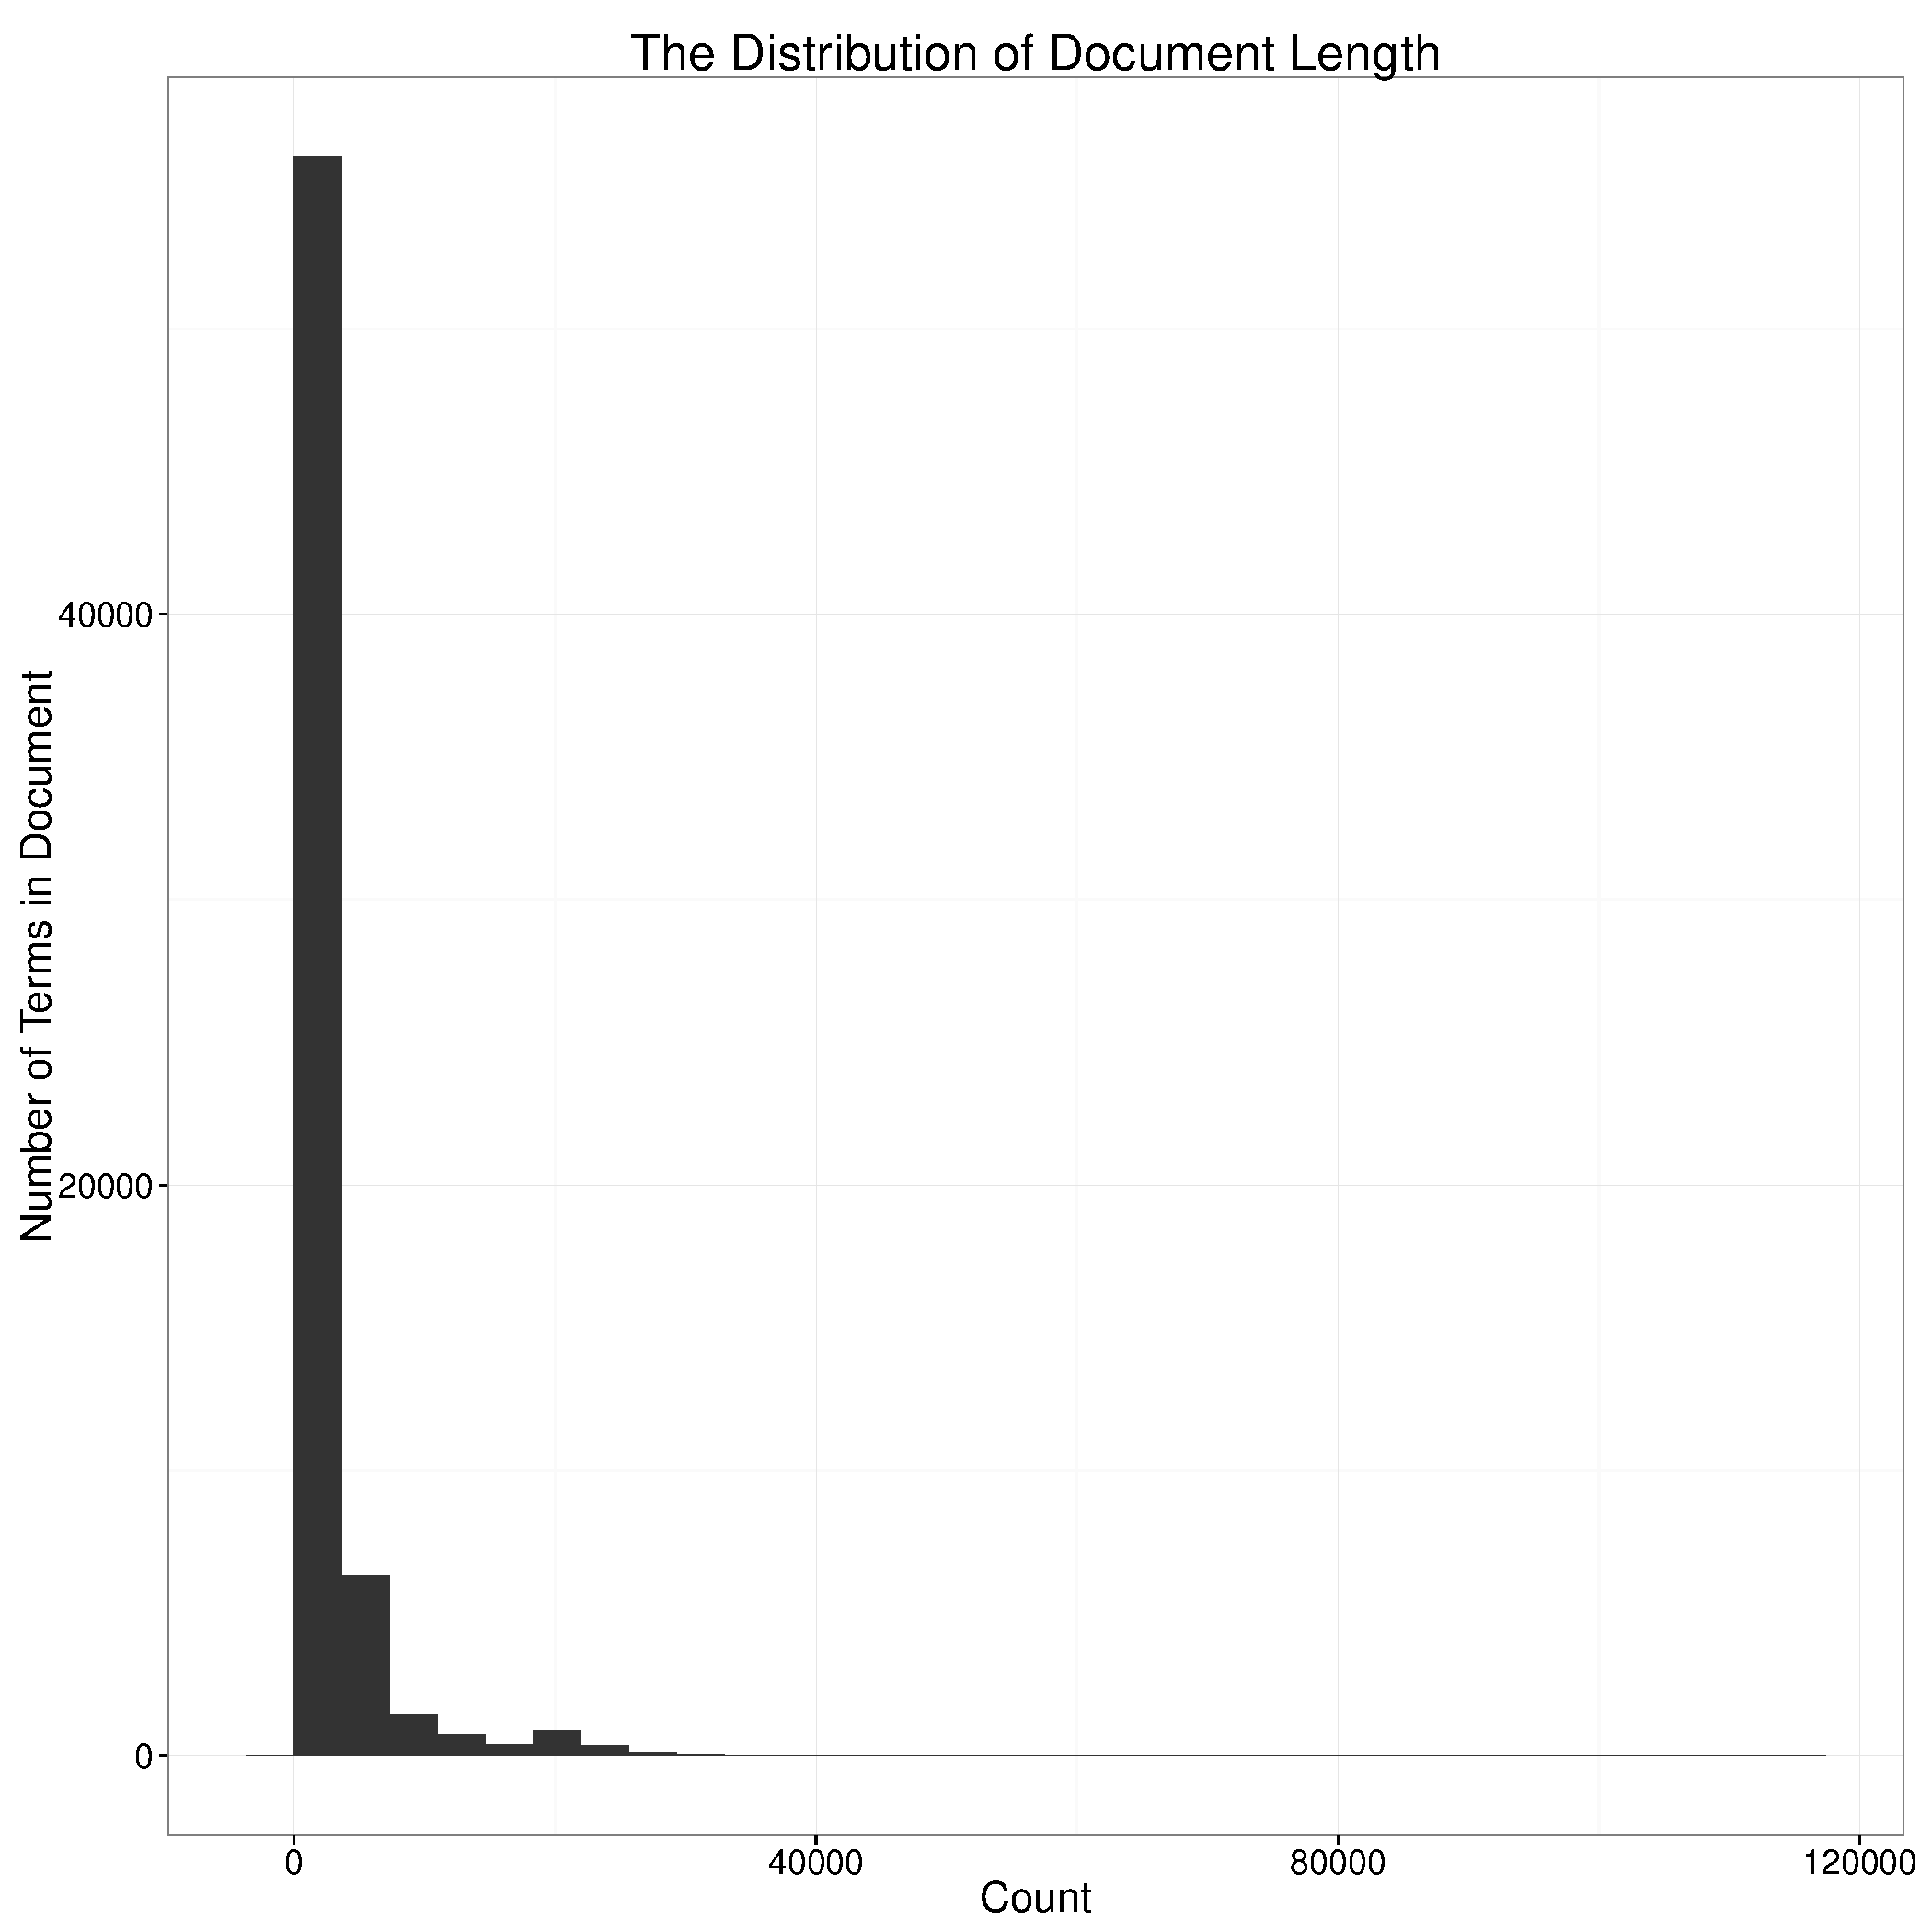
\includegraphics{figure/Document-Lengths.pdf}
\caption{Document Lengths}
\end{figure}

\begin{figure}[htbp]
\centering
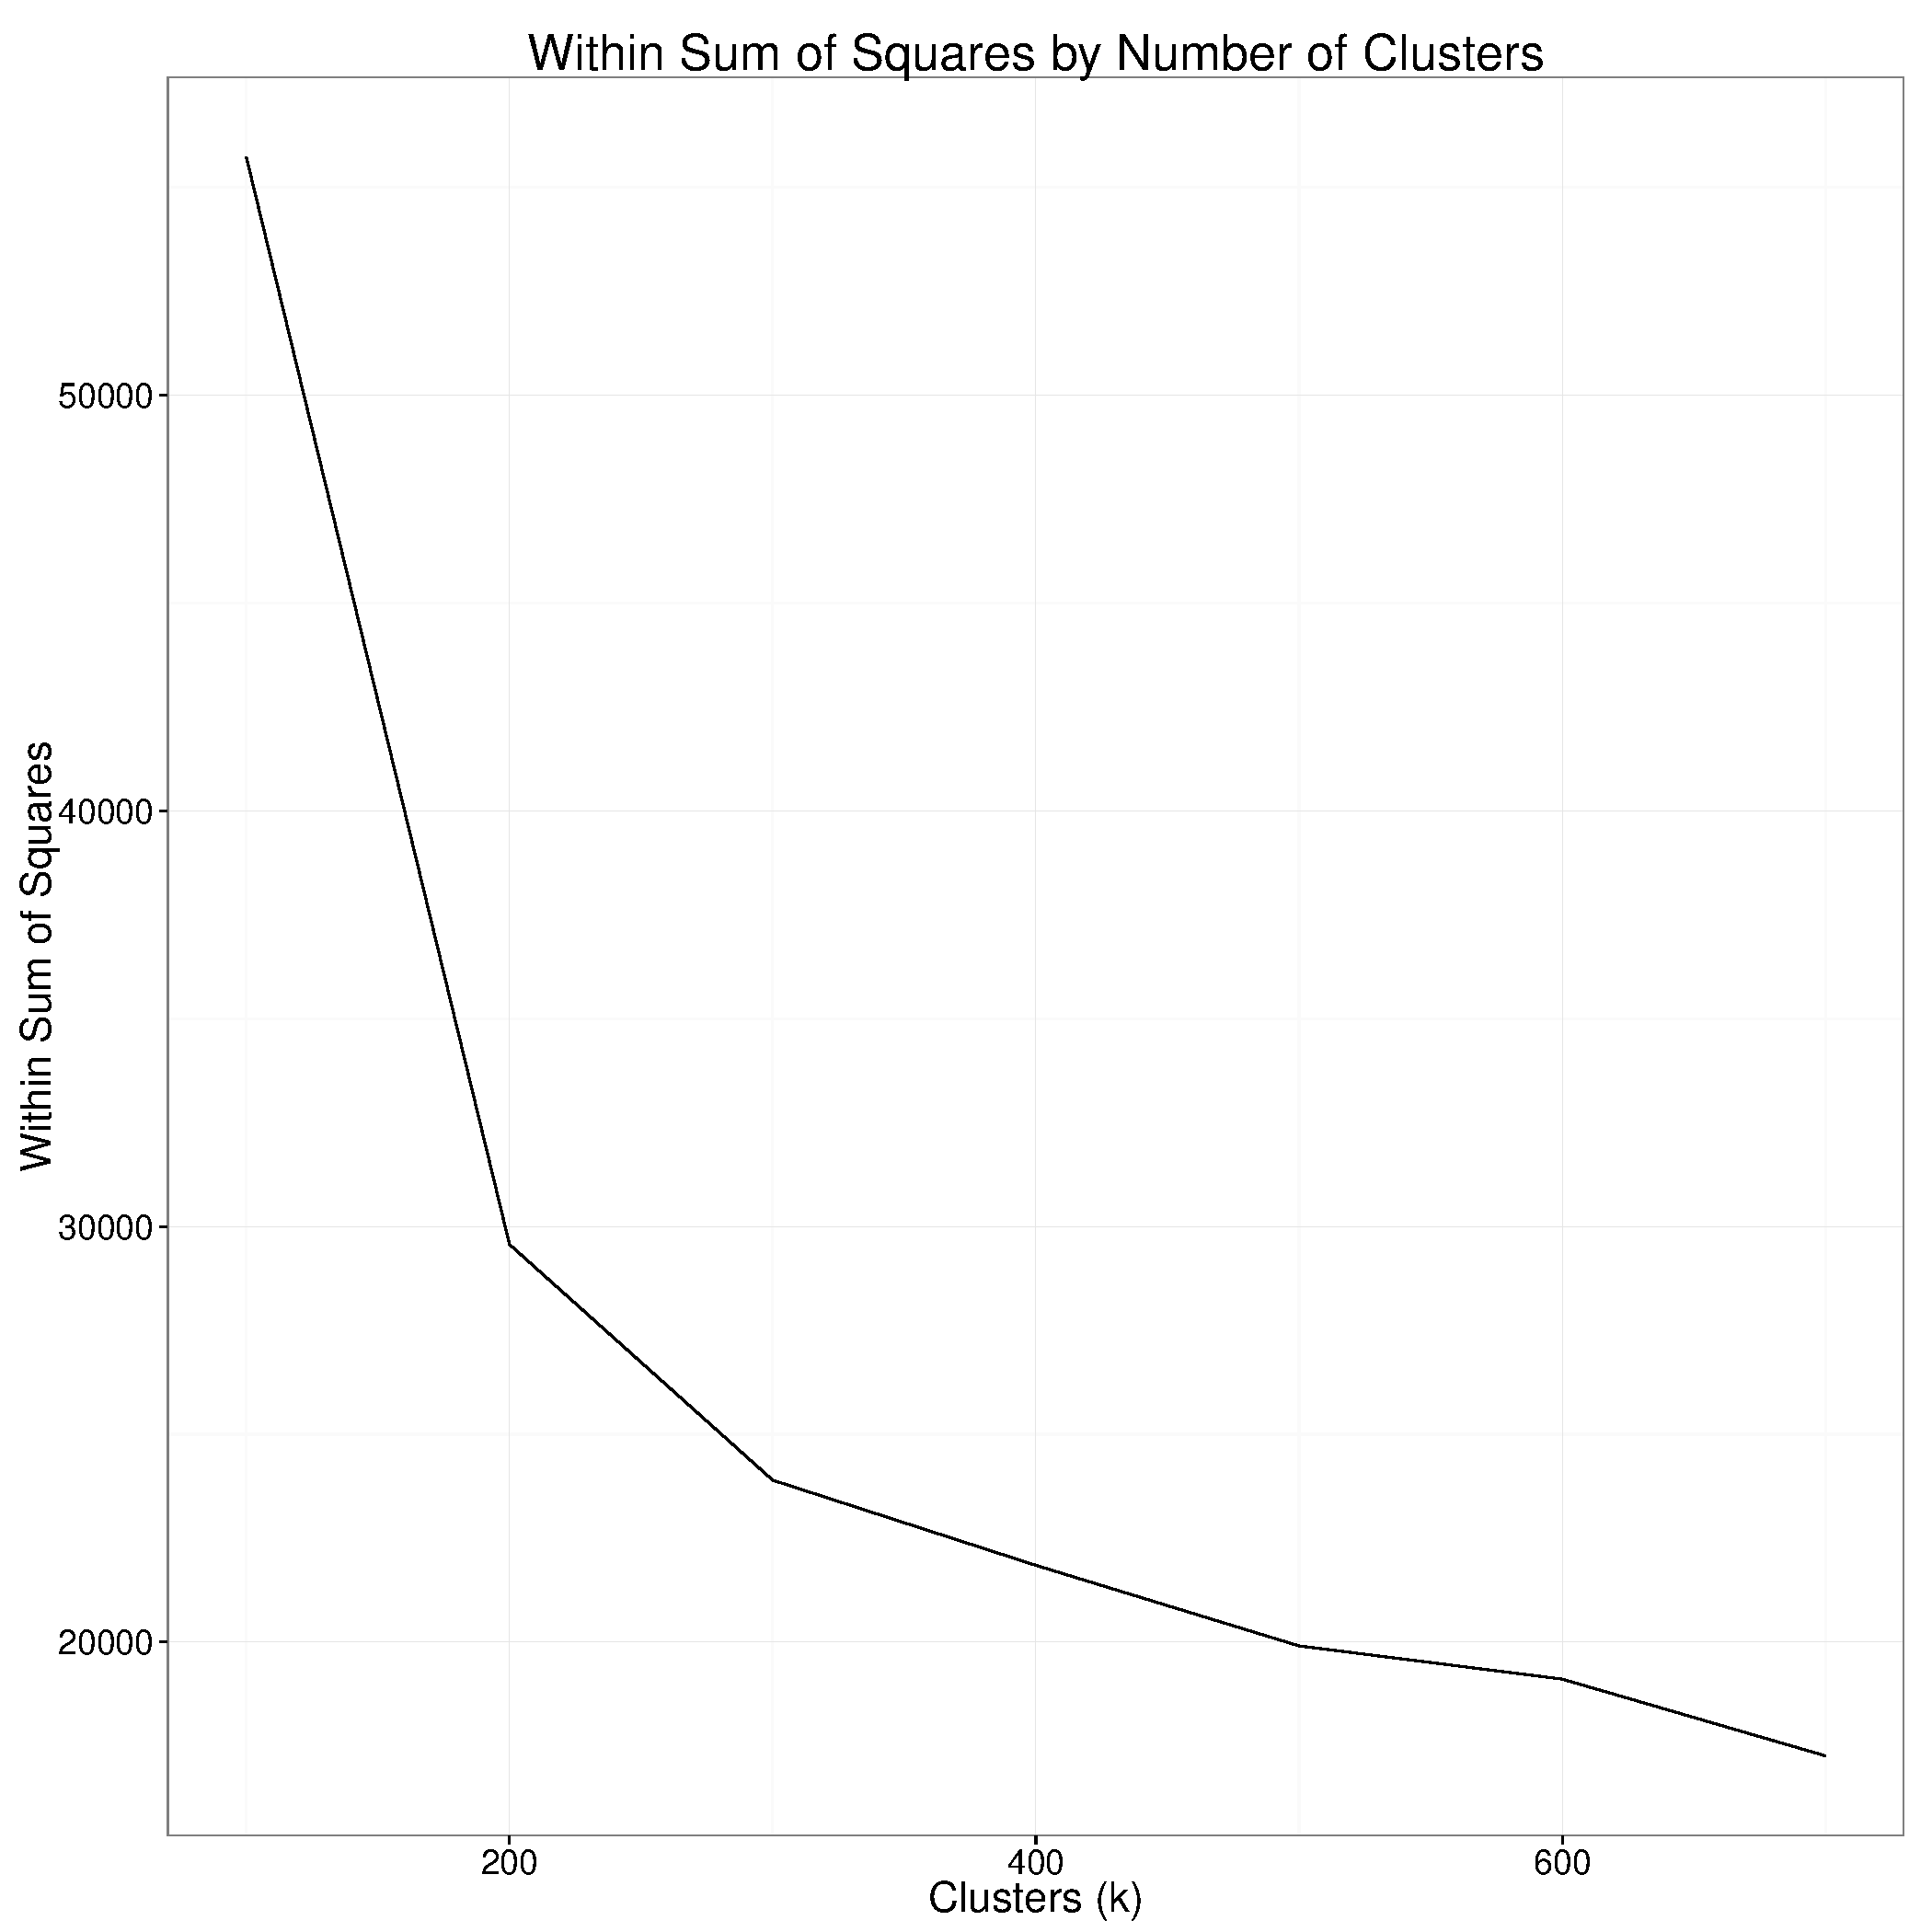
\includegraphics{figure/Cluster-Diagnostics.pdf}
\caption{Diagnostic Plot for Finding Optimal K in K-Cluster Analysis}
\end{figure}

\begin{figure}[htbp]
\centering
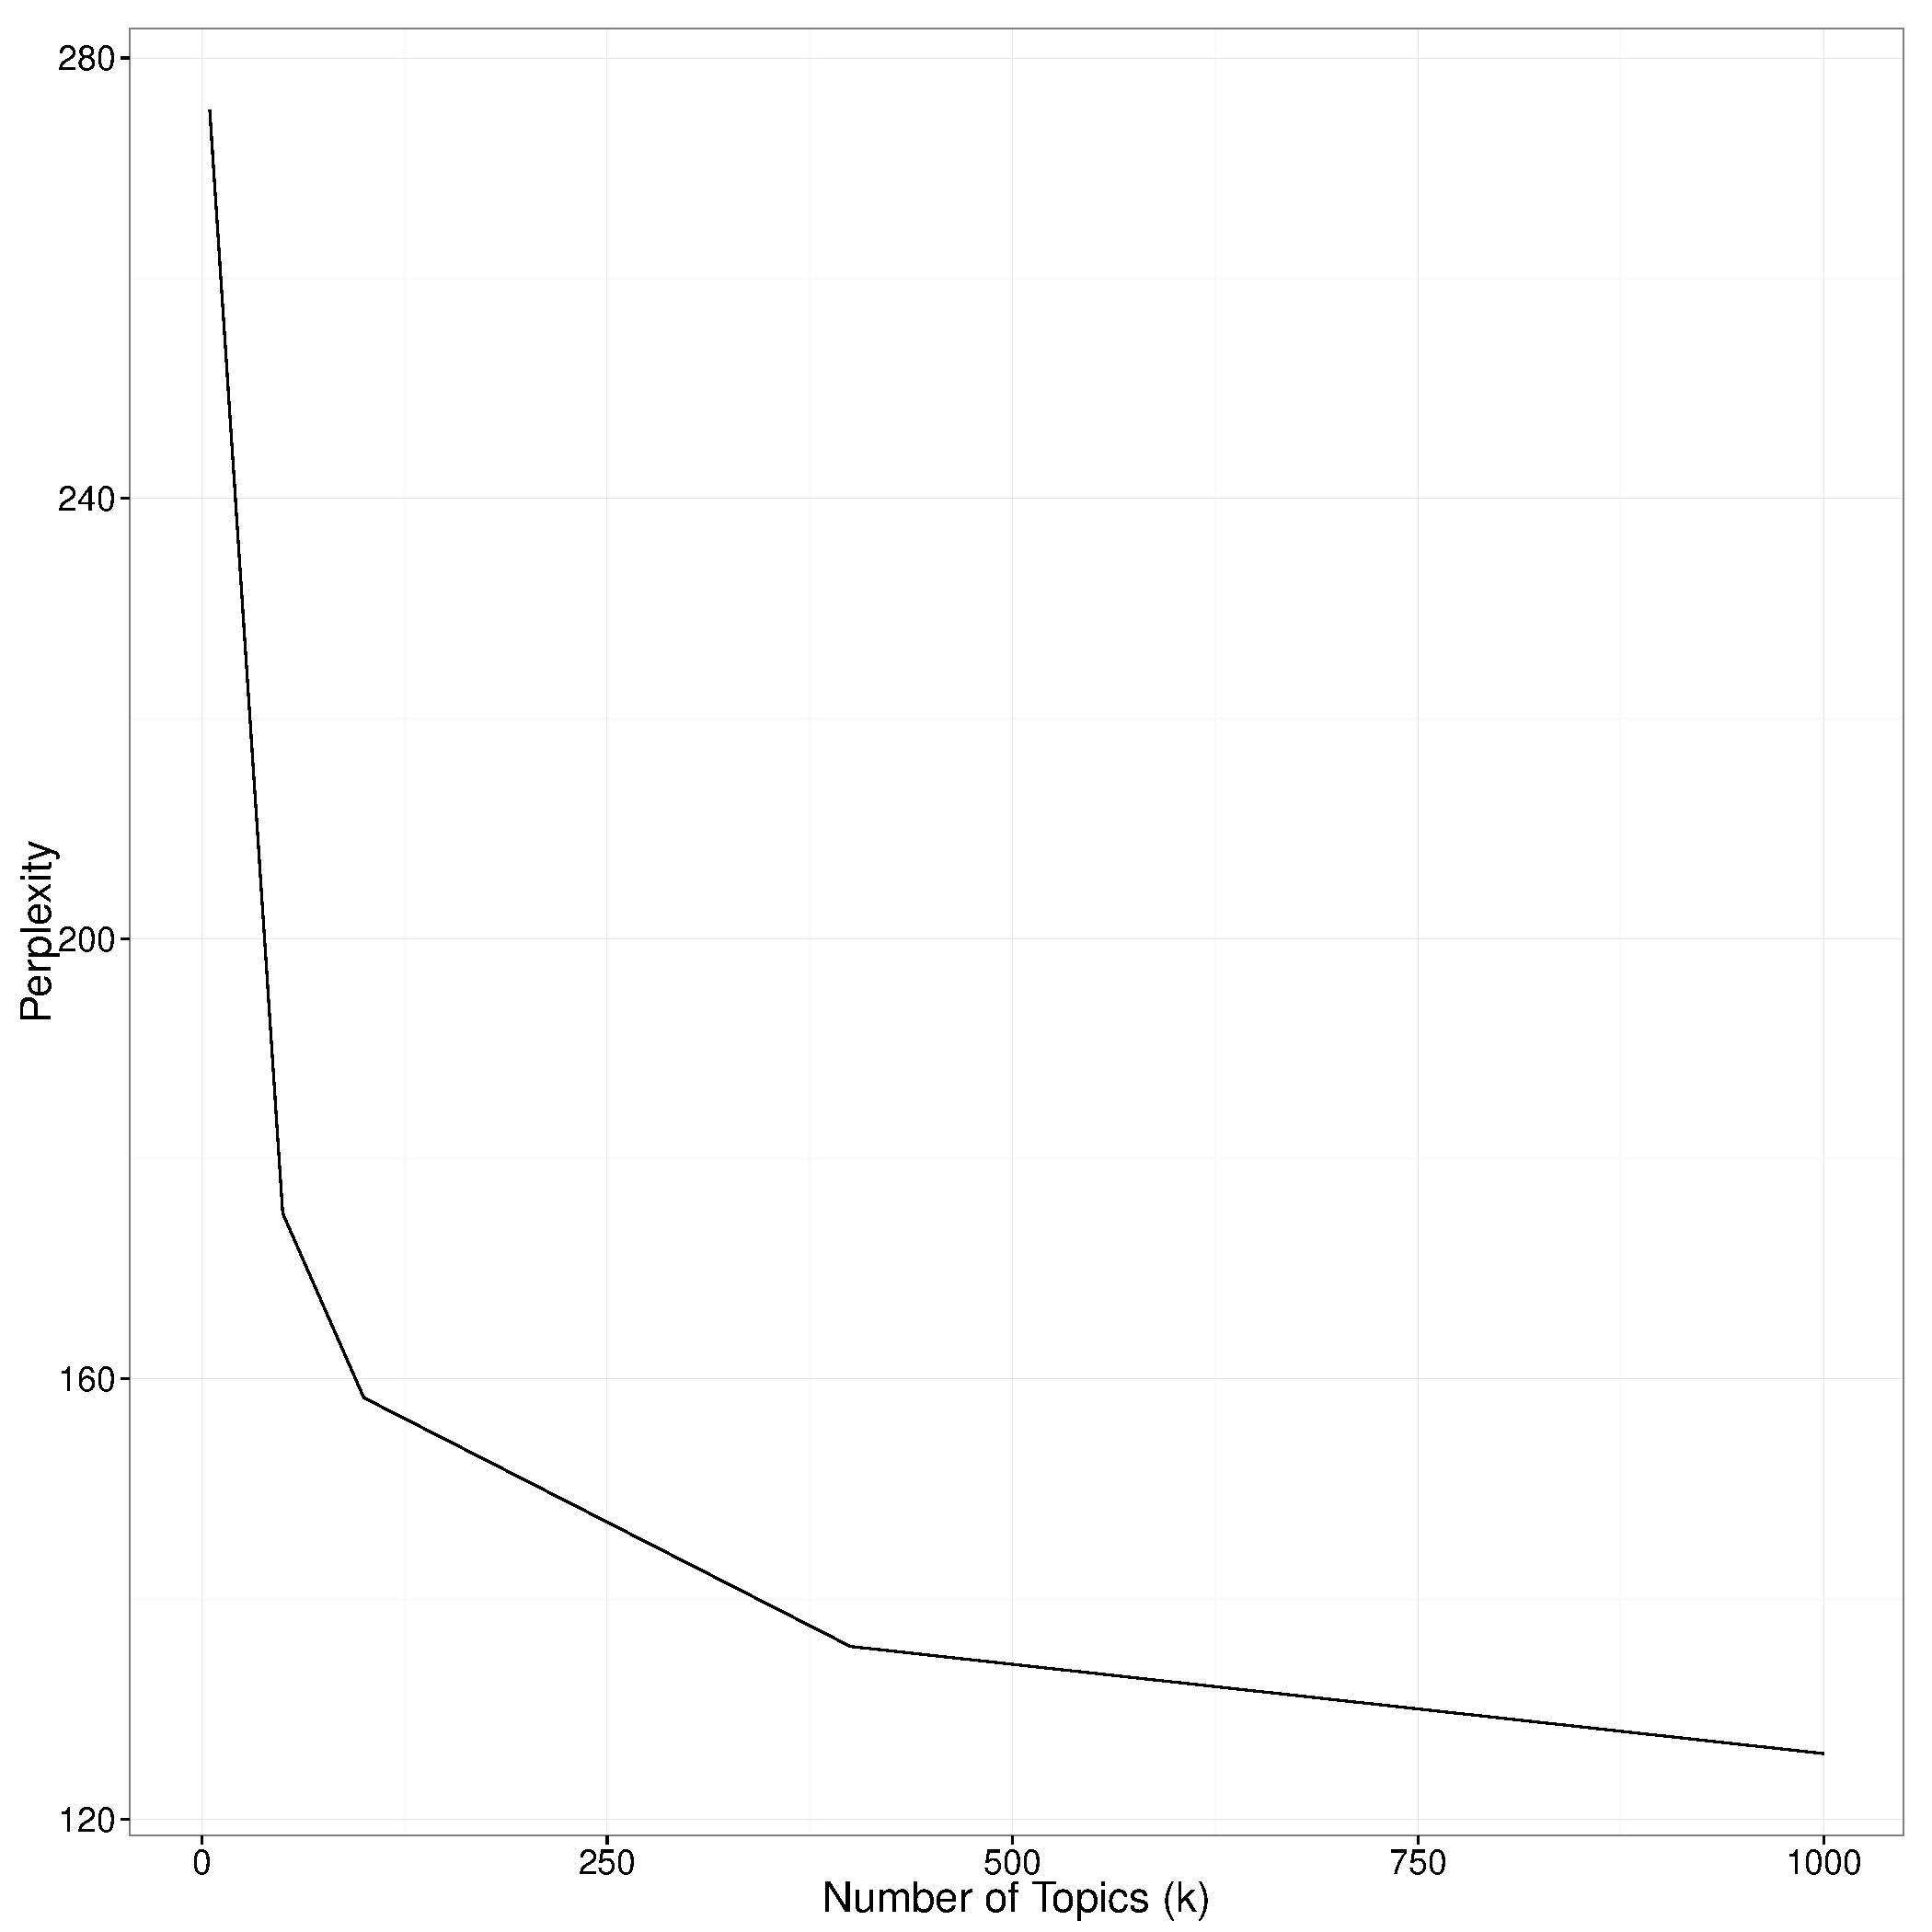
\includegraphics{figure/LDA-Diagnostics.pdf}
\caption{Diagnostic Plot for Finding Optimal Number of Topics in LDA
Topic Model}
\end{figure}

\pagebreak

\section{References}\label{references}

\setlength{\parindent}{-0.2in} \setlength{\leftskip}{0.2in}
\setlength{\parskip}{8pt} \vspace*{-0.2in} \noindent

Hay, Colin, and Ben Rosamond. 2011. ``Globalization, European
Integration and the Discursive Construction of Economic Imperatives.''
\emph{Journal of European Public Policy} 9(2): 147--67.
\url{http://www.tandfonline.com/doi/abs/10.1080/13501760110120192}.


\end{document}